\documentclass[../../main.tex]{subfiles}

\begin{document}
A continuación, describimos las diferentes arquitecturas de redes neuronales que
utilizamos durante los experimentos y los valores particulares que fueron incluidos en la
búsqueda de hiperparámetros.

Un aspecto a notar sobre nuestros datos es que contienen características temporales (la
serie de tiempo) y ``estáticas'' (el inicio de programa). Lo que hicimos en todas las
arquitecturas fue procesar la serie temporal por un lado y para hacer la clasificación,
combinar el resultado de este procesamiento con la entrada estática.

La salida de cada modelo es un número real que representa la probabilidad que la entrada
dada pertenezca a la categoría con etiqueta 1, que en nuestro caso simboliza el pertencer
al grupo de control. Para obtener la clase final (0 o 1),  se aplica un \textbf{umbral de
decisión} sobre esta probabilidad: si la probabilidad es mayor que dicho umbral, se
considera que el modelo ha clasificado a la entrada como pertenceciente a la clase 1. En
nuestro caso, fijamos este umbral en 0.5.

Dejamos algunos hiperparámetros fijos en todas los modelos:
\begin{itemize}[itemsep=0cm, topsep=0cm, parsep=0cm, partopsep=0cm]
    \item Número de épocas: 100.
    \item Número de capas: 2.
    \item Optimizador: Adam.
\end{itemize}

Y aquellos sobre los que llevamos a cabo una búsqueda son:
\begin{itemize}[itemsep=0cm, topsep=0cm, parsep=0cm, partopsep=0cm]
    \item Tamaño de lote.
    \item Número de neuronas por capa.
    \item Tasa de aprendizaje.
\end{itemize}

\subsection{Arquitectura 1: Red LSTM}
\begin{figure}[H]
    \centering
    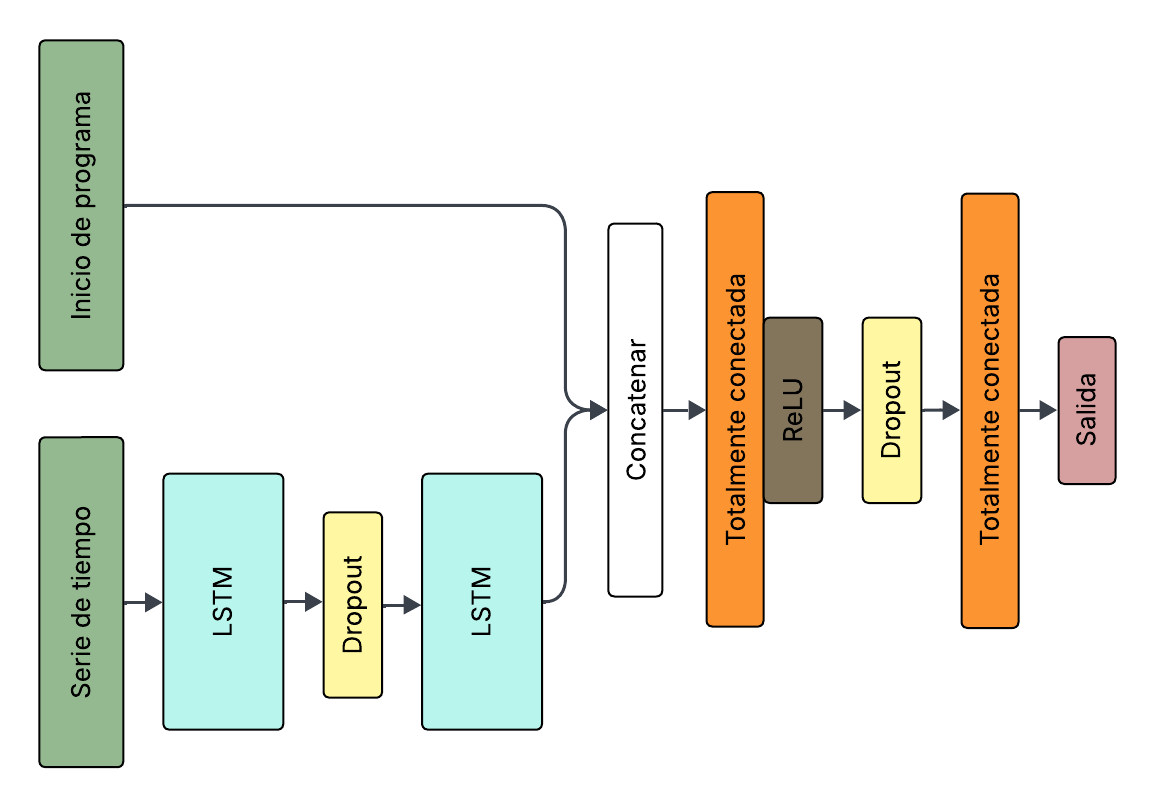
\includegraphics[width=0.7\textwidth]{figs/lstm_v2.png}
    \caption{Esquema de la arquitectura de la red LSTM propuesta.}
    \label{fig:lstm_v2}
\end{figure}

\subsection{Arquitectura 2: Red Convolucional}
\begin{figure}[H]
    \centering
    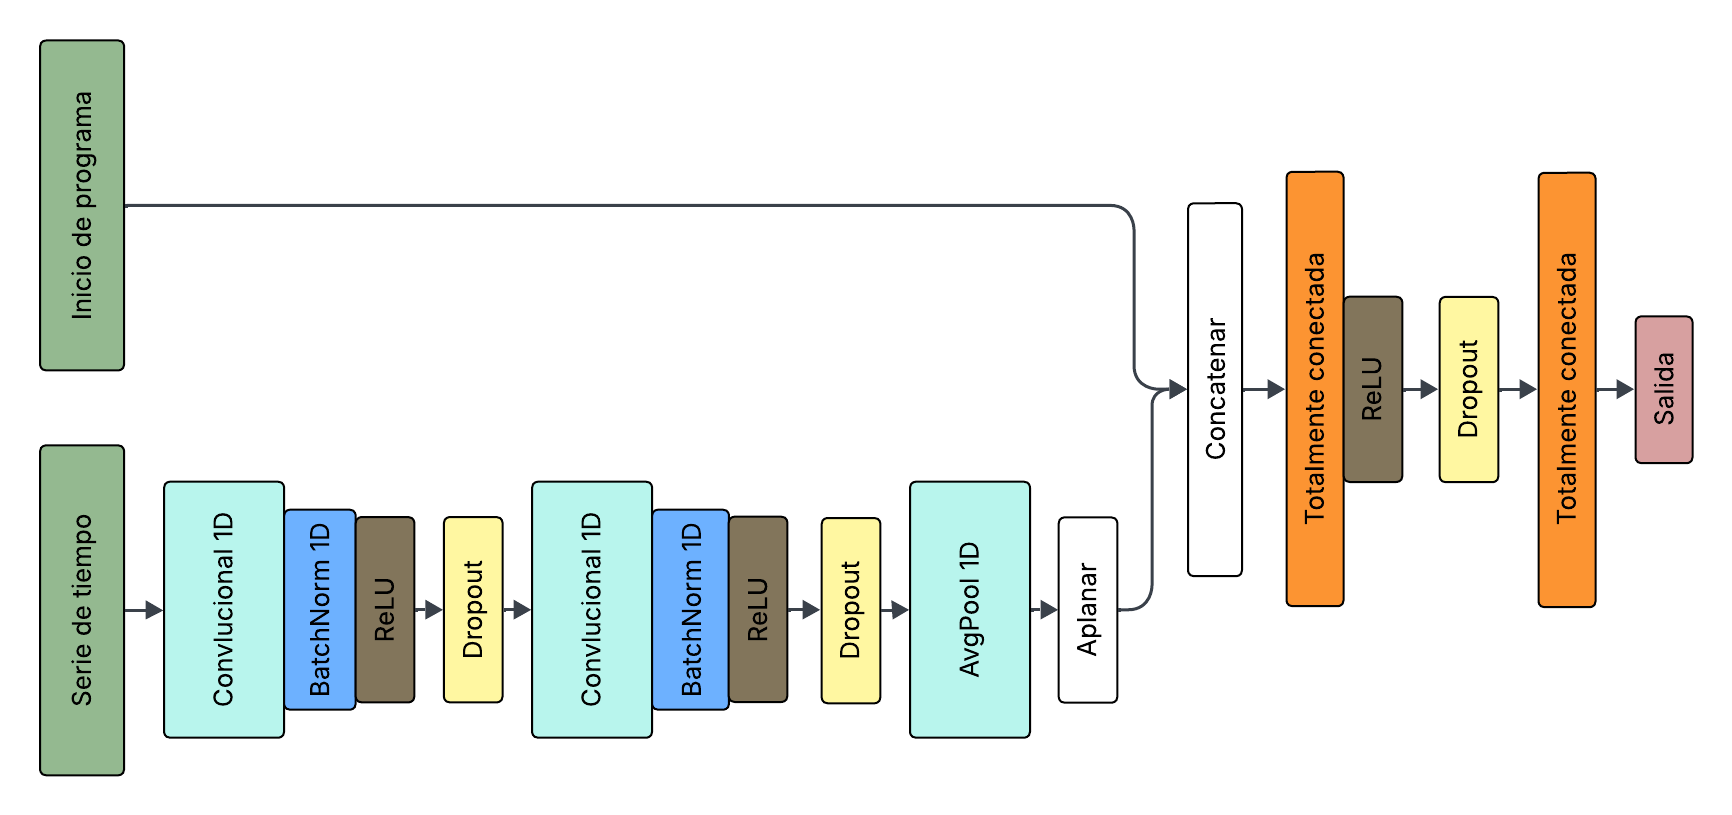
\includegraphics[width=0.8\textwidth]{figs/conv.png}
    \caption{Esquema de la arquitectura de la red convolucional propuesta.}
    \label{fig:conv}
\end{figure}


\subsection{Arquitectura 3: Red Convolucional + LSTM}
\begin{figure}[H]
    \centering
    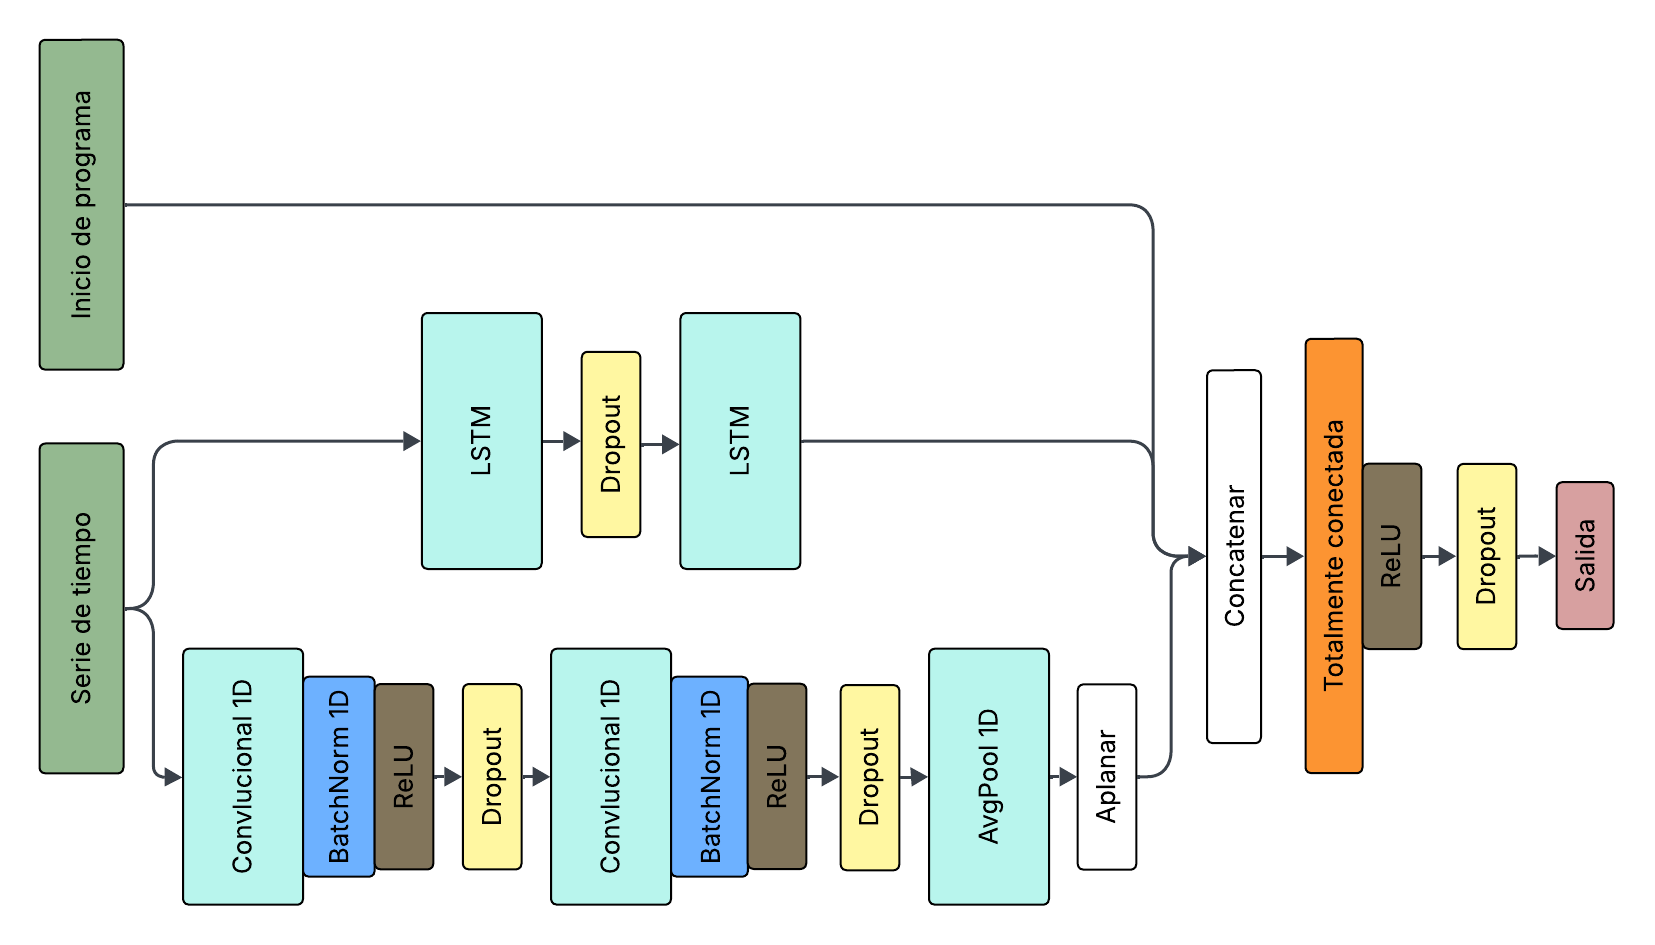
\includegraphics[width=0.8\textwidth]{figs/lstm_conv.png}
    \caption{Esquema de la arquitectura de la red LSTM + convolucional propuesta.}
    \label{fig:lstm_v2_conv}
\end{figure}

\end{document}